\subsection{标量环的扩张}

设A，A'为两个交换环，且 \(\rho:A\to A'\) 为一个环同态。设M为一个A-模，M'为一个A'-模，且 \(u:M\to M'\) 为一个A-同态；由于典范单射 \(\phi_{M'}:M'\to T_{A'}(M')\) （通过标量限制）也是一个A-同态，所以复合映射 \(M\xrightarrow{u}M'\xrightarrow{\phi_{M'}}T_{A'}(M')\) 也是A-同态。由（第 2 号）导出一个 A-代数同态 \(T_{A}(M)\to\rho*(T_{A'}(M'))\) ，也记为 \(T(u):T_{A}(M)\to T_{A'}(M')\) ，它是使图表交换的唯一 A-同态。

\begin{enumerate}
\def\labelenumi{(\arabic{enumi})}
\setcounter{enumi}{7}
\tightlist
\item
\end{enumerate}

\pandocbounded{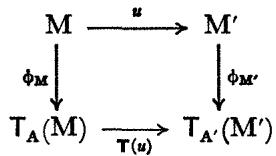
\includegraphics[keepaspectratio]{images/part003_9672ae23.jpg}}

若 \(\sigma: \mathbf{A}' \to \mathbf{A}''\) 是一个交换环同态， \(\mathbf{M}''\) 是一个 \(\mathbf{A}''\) -模，且 \(v: \mathbf{M}' \to \mathbf{M}''\) 是一个 \(\mathbf{A}'\) -同态，则上述唯一性性质表明

\[
\mathbf {T} (v \circ u) = \mathbf {T} (v) \circ \mathbf {T} (u).\tag{9}
\]

命题5. 设A，B为两个交换环， \(\rho: \mathbf{A} \to \mathbf{B}\) 一个环同态，且 M 是一个 A-模。典范扩张

\[
\psi : \mathsf {T} _ {\mathbf {B}} (\mathbf {B} \otimes_ {\mathbf {A}} \mathbf {M}) \rightarrow \mathbf {B} \otimes_ {\mathbf {A}} \mathsf {T} _ {\mathbf {A}} (\mathbf {M})
\]

（它是 B-线性映射 \(\mathbf{1}_{\mathbf{B}} \otimes \phi_{\mathbf{M}}: \mathbf{B} \otimes_{\mathbf{A}} \mathbf{M} \to \mathbf{B} \otimes_{\mathbf{A}} \mathsf{T}_{\mathbf{A}}(\mathbf{M})\) 的典范扩张）是分次 B-代数的同构。

考虑两个A-代数同态：典范单射 \(j: \mathbf{B} = \mathsf{T}^0(\mathbf{B} \otimes_{\mathbf{A}} \mathbf{M}) \to \mathsf{T}(\mathbf{B} \otimes_{\mathbf{A}} \mathbf{M})\) 及同态

\[
h = \mathsf {T} (i): \mathsf {T} (\mathbf {M}) \rightarrow \mathsf {T} (\mathbf {B} \otimes_ {\mathbf {A}} \mathbf {M})
\]

由典范 A-线性映射导出（参见公式 (8)），

\[
i: \mathbf {M} \rightarrow \mathbf {B} \otimes_ {\mathbf {A}} \mathbf {M}.
\]

由于 \(\mathsf{T}^0 (\mathbf{B}\otimes_{\mathbf{A}}\mathbf{M})\) 包含于 \(\mathsf{T}(\mathbf{B}\otimes_{\mathbf{A}}\mathbf{M})\) 的中心，可以应用 §4 第 2 号的命题 5，从而得到一个 A-代数同态

\[
\psi^ {\prime}: \mathbf {B} \otimes_ {\mathbf {A}} \mathsf {T} (\mathbf {M}) \rightarrow \mathsf {T} (\mathbf {B} \otimes_ {\mathbf {A}} \mathbf {M})
\]

，使得对于 \(\beta \in \mathbf{B}\) , \(x_{i} \in \mathbf{M}\) （ \(1 \leqslant i \leqslant n\) ），

\[
\psi^ {\prime} (\beta \otimes (x _ {1} \otimes x _ {2} \otimes \dots \otimes x _ {n})) = \beta ((1 \otimes x _ {1}) \otimes (1 \otimes x _ {2}) \otimes \dots \otimes (1 \otimes x _ {n})),
\]

这立即表明 \(\psi'\) 也是一个B-代数同态。只需证明 \(\psi \circ \psi'\) 和 \(\psi' \circ \psi\) 分别是 \(B \otimes_{A} T(M)\) 和 \(T(B \otimes_{A} M)\) 上的恒等映射。现在，这两个代数都由 \(B \otimes_{A} M\) 生成，并且显然 \(\psi \circ \psi'\) 和 \(\psi' \circ \psi\) 与 \(B \otimes_{A} M\) 上的恒等映射一致，由此得出结论。

